%----------------------------------------------------------------------------
\chapter{\bevezetes}
%----------------------------------------------------------------------------

\section{Motivation}
Navigation of mobile robots has been a very active research area worldwide. It is essential for these autonomous vehicles to thoroughly explore their surroundings before starting their tasks. It is not advised for any of them to go wandering in their environment because they will get lost or bump into obstacles.

One of the simplest examples of an autonomous agent is a robot vacuum cleaner. I can provide some firsthand experiences, because I own an iRobot Roomba 780 and my parents own an iRobot Roomba i7. The 780 is an older model from 2010, it just wanders from wall to wall in the house, it does not perform any localization or mapping, it measures its movements simply based on the wheel rotations, and it turns around when it bumps into an object. On the other hand, the i7 has a camera on top (even though it is of very low resolution for privacy reasons), which can see the ceiling of the rooms. At the first run, the robot executes an autonomous mapping sequence, so it goes around in the rooms and maps out the space. After the mapping has finished, we can see the map of the apartment in the companion app. The i7 is much more flexible, because it knows where its docking station is located, it can distinguish individual rooms, and it can localize itself in the apartment, and so it can vacuum systematically.

\begin{figure}[H]
	\centering
	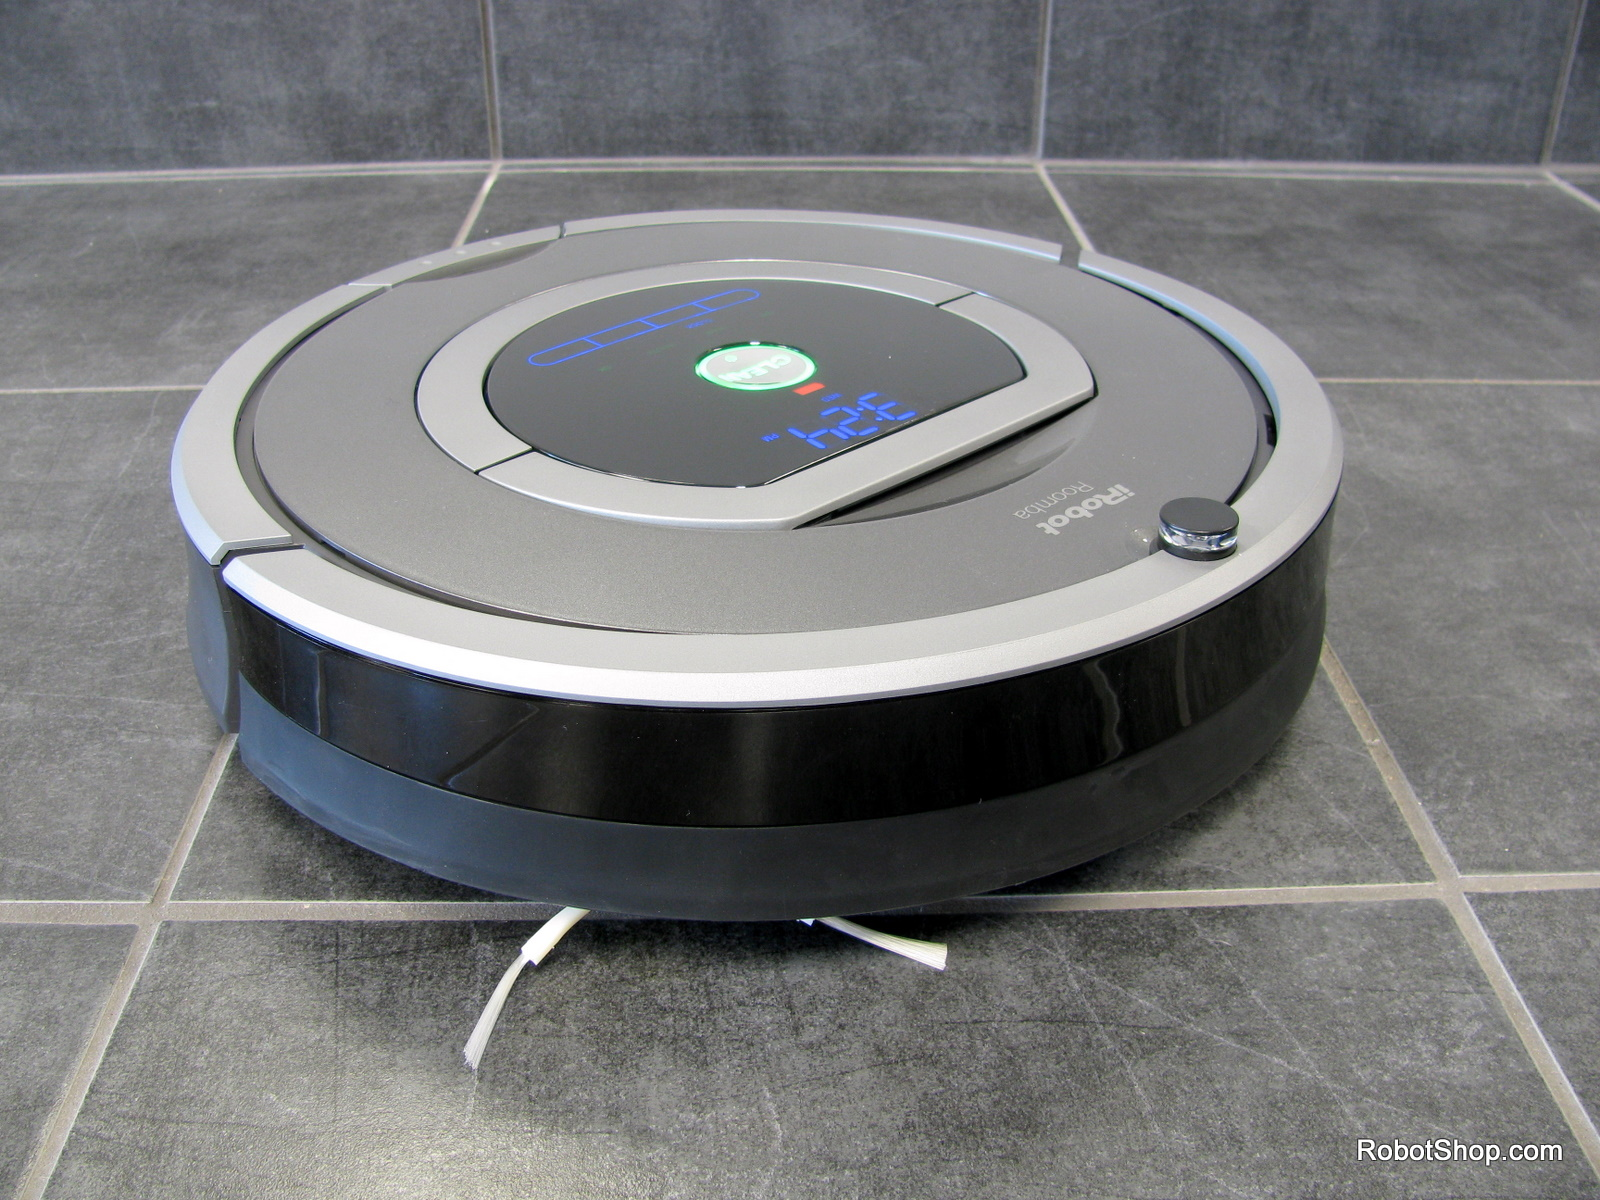
\includegraphics[width=67mm, keepaspectratio]{figures/iRobot_roomba_780.jpg}\hspace{1cm}
	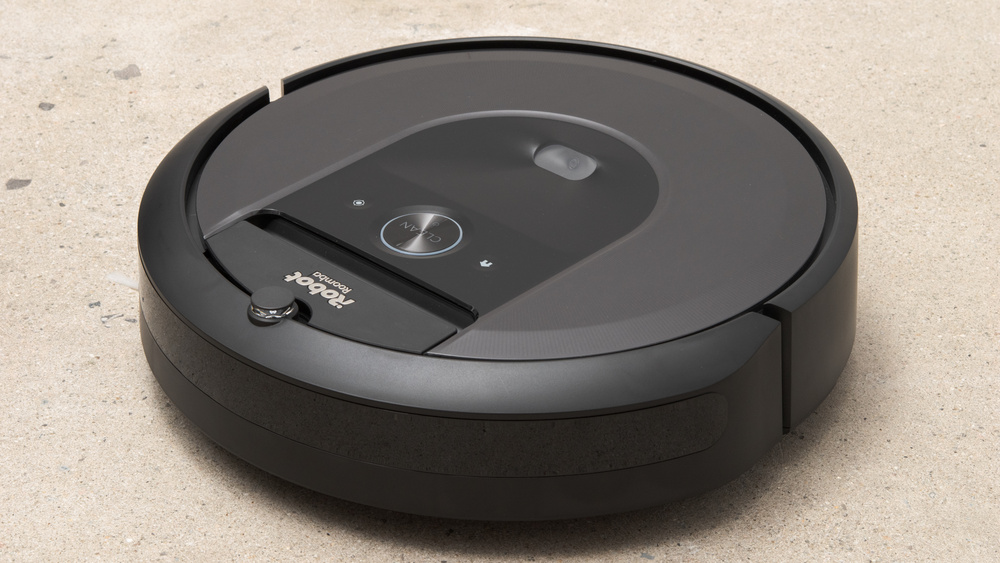
\includegraphics[width=67mm, keepaspectratio]{figures/iRobot_roomba_i7.jpg}\\\vspace{5mm}
	\caption{iRobot Roomba 780 (left) and i7 (right) (sources: \cite{roomba780}\cite{roombai7})}
	\label{fig:Roombas}
\end{figure}

As this illustrative example shows, the advantages of SLAM (simultaneous localization and mapping) in a housekeeping environment is clear. Mobile robots and SLAM can be used in various industrial environments too. For example, autonomous robots can carry heavy products from one place to another in a huge warehouse. In these cases it is unimaginable that a wall-to-wall algorithm could achieve efficient navigation (it is questionable if it would even arrive to its goal before draining its battery). All in all, nowadays it is very important to use some SLAM algorithm.

\section{Goal of the thesis}

The aim of this thesis is to further develop the navigation and exploration capabilities of a mobile robot, so that it can independently explore its surroundings when it arrives at a new location and create a map. This map could be reused by it or other robots.

The main goal is to use V-SLAM (Visual-SLAM) with a stereo camera instead of SLAM with a LIDAR. The reasons behind this choice are:
\begin{itemize}
\setlength\itemsep{0em}
    \item a camera can easily build 3D maps or point clouds of the robots' surroundings,
    \item if the camera has RGB lenses than we can create colorful point clouds of its environment,
    \item the camera can be used to detect and recognize objects.
\end{itemize}
One of our goals was to detect persons with the camera and prepare the robot to be able to follow or avoid them.

\section{Structure of the thesis}

During the first semester of my thesis project, I have gained significant experience in many fields. First, I learned about mobile robots, OAK-D cameras and neural reconstruction in Chapter~\ref{related_works}, then I digged deeper in the capabilities of the OAK-D camera in Chapter~\ref{experiments_oak_d}, experimented with NeRFs and Gaussian Splatting in Chapter~\ref{nerf_gsplat}. After these I gained experience in 3D mapping using RTAB-Map, nvblox and Isaac VSLAM in Chapter~\ref{experiments_3d_mapping}. Then, I started the implementation of the mapping and the person detector in Chapter~\ref{implementation}. Last but not least we suggested some future plans for the next semester in Chapter~\ref{future_plans}.
